%---------------------------------------------------------
%	Packages and doc config
%---------------------------------------------------------

\documentclass{report}

% \setlength\parindent{0pt} % Removes all indentation from paragraphs

\usepackage[table]{xcolor}% http://ctan.org/pkg/xcolor

\usepackage[english]{babel}

\usepackage[english]{babel}
\usepackage[utf8]{inputenc}
\usepackage[margin=3cm]{geometry}
\usepackage{graphicx}
\usepackage{todonotes}
\usepackage{float}
\usepackage{amsmath}
\usepackage{subcaption}
\usepackage{listings}
\usepackage{color}
\usepackage{wrapfig}
\usepackage{titling}
\usepackage{multicol}
\usepackage{amsmath}


\renewcommand{\lstlistingname}{Code Snippet}

\lstdefinestyle{customc}{
  belowcaptionskip=1\baselineskip,
  breaklines=true,
  language=C,
  showstringspaces=false,
  basicstyle=\ttfamily,
  keywordstyle=\bfseries\color{green!40!black},
  commentstyle=\itshape\color{purple!40!black},
  identifierstyle=\color{blue},
  stringstyle=\color{orange},
}

\lstdefinestyle{customv}{
  belowcaptionskip=1\baselineskip,
  breaklines=true,
  showstringspaces=false,
  basicstyle=\footnotesize\ttfamily,
}

%\usepackage{times} % Uncomment to use the Times New Roman font

%---------------------------------------------------------
%	Document
%---------------------------------------------------------

\title{CM30225 Parallel Computing\\Shared Memory} % Title
\author{Rowan Walshe} % Author name

\date{\today} % Date for the report

\begin{document}

\maketitle % Insert the title, author and date
\pagebreak

\chapter{Code}
\section{Introduction}
While working on this coursework, I attempted a number of different solutions for parallelising the problem. In this section I will discuss the different approaches to parallelism for each version, along with the advantages and disadvantages.
\section{Sequential Version}

\section{Version 1}
In the sequential program of my attempt, the program moves through the 2D array from the top left down to the bottom right. At each point it temporally stores the value at the point, then calculates the new value based on the average of the surrounding four values. It then checks to see if the absolute difference between the new and old value is greater than the given precision. If the value at any point changes more than the given precision, then at the end of this iteration of averaging values, it must complete at least one more iteration. This is illustrated in Code Snippet 1.1.
\begin{lstlisting}[style=customc,caption=Version 1 Sequential Main Loop]
    while(1) {
        endFlag = true;
        iterations++;
        for(i=1; i<sizeOfPlane-1; i++) {
            for(j=1; j<sizeOfPlane-1; j++) {
                pVal = plane[i][j];
                plane[i][j] = (plane[i-1][j] + plane[i+1][j]
                    + plane[i][j-1] + plane[i][j+1])/4;
                if(endFlag && tolerance < fabs(plane[i][j]-pVal)) {
                    endFlag = false;
                }
            }
        }
        if(endFlag) {
            return iterations;
        }
    }
\end{lstlisting}
To parallelise this, each thread is given a certain number of rows that it has calculate. The threads work out which rows of the 2D array they have to work on based on the size of the 2D array, the total number of threads and their thread ID. For example if the 2D array is of size 10 by 10 and there are four threads total, each thread will work on exactly two rows. If the number of rows does not divide evenly between the number of threads, and there are n rows remaining, then one extra row is given to the thread with ID's less than the number of remaining rows. This means that at most, each thread has to calculate the averages for one extra row. The logic for this can be found in Code Snippet 1.2.
\begin{lstlisting}[style=customc,caption=Row Split Logic]
    unsigned int sizeOfInner = threadData->sizeOfPlane-2;
    unsigned int rowsPerThreadS = sizeOfInner/threadData->threadCount+1;
    unsigned int rowsPerThreadE = sizeOfInner/threadData->threadCount;
    unsigned int remainingRows = sizeOfInner - threadData->threadCount*rowsPerThreadE;

    unsigned int startingRow, endingRow;
    if(threadData->id < remainingRows) {
        startingRow = threadData->id * rowsPerThreadS + 1;
        endingRow = startingRow + rowsPerThreadS;
    } else {
        startingRow = threadData->id * rowsPerThreadE + remainingRows + 1;
        endingRow = startingRow + rowsPerThreadE;
    }
\end{lstlisting}
After a thread has done their portion of the work, they barrier once to wait for all of the threads to finish doing their work on the 2D array. Then each thread checks to see if they need to do another iteration or not. Once they have checked barrier again. The main thread then resets the finished flag, followed by one more barrier. If the threads did not barrier to wait for all the threads to finish their calculations, you end up with a race condition, and some threads may attempt to prematurely return, which would cause the program to freeze. If the threads did not barrier before reseting the finished flag, the flag may be reset before all of the threads have checked whether or not they have finished or not which would be a race condition, and would lead to a similar situation as before. Finally, they barrier once after the flag has been reset, so that the threads do not start work early, which would be a race condition, that may lead to incorrect results. The code for the main loop of the main thread can be found in Code Snippet 1.3. The only difference from the main loop of the child threads is that it counts the number of iterations, and it is the only thread that attempts to reset the finished flag.
\begin{lstlisting}[style=customc,caption=Version 1 Parallel Main Loop]
    while(1) {
        iterations++;

        relaxPlaneRows(threadData->plane, threadData->sizeOfPlane, threadData->tolerance, startingRow, endingRow);

        pthread_barrier_wait(&barrierGeneric);
        if(finishedFlag)
            return iterations;
        pthread_barrier_wait(&barrierGeneric);
        finishedFlag = true;
        pthread_barrier_wait(&barrierGeneric);
    }
\end{lstlisting}
While this solution is relatively simple and scales pretty well as can be seen in my scalability testing, it is not particularly fast, with later versions reducing the time it takes to run by upwards of 60\%. One of the downsides of this solution is that you may get slightly different results run to run, when using more than one thread. This is because when a thread reaches a row on the boundary between the rows that it has to work on and the rows that another thread is working on, instead of getting update averages above and to the left of it, it now also gets update averages from the row bellow as well. This means that the sequential and parallel versions of this solution are not really the same algorithm. This means that it may also be harder to prove correctness of the solution.
\section{MPI Version}
\begin{wrapfigure}{r}{0.35\textwidth}
\vspace{-30pt}

\includegraphics[width=0.35\textwidth]{checkerboard}
\caption{Chequerboard Pattern}
\label{fig:subim1}
\end{wrapfigure}
The goal with my second version was to come up with a way of traversing the 2D array so that no matter the number of threads that the program was using, it would not affect the solution. My idea was to traverse over the 2D array in a chequerboard patter. This would add some overheads as in the parallel version, you would have to barrier after calculating the average of half of the points in the 2D array, as well as at the end. However, on top of having the added benefit of making correctness testing much easier, it also decreased the time it took to run from my first version by upwards of 50\%. The code for the main loop of the sequential program can be found in Snippet 1.4.
\\
\begin{lstlisting}[style=customc,caption=Version 2 Sequential Main Loop]
    while(1) {
        finishedFlag = true;
        iterations++;
        for(i=1; i<sizeOfPlane-1; i++) {
            relaxRow(plane, sizeOfPlane, tolerance, i, (i%2)+1);
        }
        for(i=1; i<sizeOfPlane-1; i++) {
            relaxRow(plane, sizeOfPlane, tolerance, i, ((i+1)%2)+1);
        }
        if(finishedFlag) {
            return iterations;
        }
    }
\end{lstlisting}
With this version I created a function \textit{relaxRow} that calculates the new averages for every other value in row \textit{i} starting from the first or second value along in the row depending on which part of the chequerboard is currently being relaxed. The code for the main loop of the parallel version can be found in Snippet 1.5. It bears similarities to the parallel main loop of version one, except now there are four barriers as there is a new barrier half way through the relaxation process.
\\\\\\\\
\begin{lstlisting}[style=customc,caption=Version 2 Parallel Main Loop]
    while(1) {
        iterations++;
        for(row=startingRow; row<endingRow; row++) {
            relaxPlaneRow(threadData->plane, threadData->sizeOfPlane, threadData->tolerance, row, (row%2)+1);
        }
        // Barrier for first half of chequerboard
        pthread_barrier_wait(&barrierGeneric);        
        for(row=startingRow; row<endingRow; row++) {
            relaxPlaneRow(threadData->plane, threadData->sizeOfPlane, threadData->tolerance, row, ((row+1)%2)+1);
        }
        // Barrier for second half of chequerboard
        pthread_barrier_wait(&barrierGeneric);
        if(finishedFlag) {
            return iterations;
        }
        pthread_barrier_wait(&barrierGeneric);
        finishedFlag = true;
        pthread_barrier_wait(&barrierGeneric);
    }
\end{lstlisting}

As the number of iterations that it has to complete is very similar if not sometimes more than my original version, it is not immediately obvious why this version performs so much better. However by using the cachegrind tool in valgrind, you are able to see that my second version has an L1 data cache miss rate that is less than half that of my first version.

\begin{lstlisting}[style=customv,caption=Version 1 Cachegrind]
==65481== I   refs:      59,145,477,672
==65481== I1  misses:             1,217
==65481== LLi misses:             1,193
==65481== I1  miss rate:           0.00%
==65481== LLi miss rate:           0.00%
==65481==
==65481== D   refs:      27,793,013,948  (24,735,366,146 rd   + 3,057,647,802 wr)
==65481== D1  misses:       782,506,106  (   782,493,703 rd   +        12,403 wr)
==65481== LLd misses:            14,256  (         2,163 rd   +        12,093 wr)
==65481== D1  miss rate:            2.8% (           3.1%     +           0.0%  )
==65481== LLd miss rate:            0.0% (           0.0%     +           0.0%  )
==65481==
==65481== LL refs:          782,507,323  (   782,494,920 rd   +        12,403 wr)
==65481== LL misses:             15,449  (         3,356 rd   +        12,093 wr)
==65481== LL miss rate:             0.0% (           0.0%     +           0.0%  )
\end{lstlisting}
\begin{lstlisting}[style=customv,caption=Version 2 Cachegrind]
==23608== I   refs:      59,754,099,652
==23608== I1  misses:             1,215
==23608== LLi misses:             1,192
==23608== I1  miss rate:           0.00%
==23608== LLi miss rate:           0.00%
==23608==
==23608== D   refs:      28,044,004,225  (24,986,267,940 rd   + 3,057,736,285 wr)
==23608== D1  misses:       391,254,955  (   391,242,549 rd   +        12,406 wr)
==23608== LLd misses:            14,257  (         2,163 rd   +        12,094 wr)
==23608== D1  miss rate:            1.3% (           1.5%     +           0.0%  )
==23608== LLd miss rate:            0.0% (           0.0%     +           0.0%  )
==23608==
==23608== LL refs:          391,256,170  (   391,243,764 rd   +        12,406 wr)
==23608== LL misses:             15,449  (         3,355 rd   +        12,094 wr)
==23608== LL miss rate:             0.0% (           0.0%     +           0.0%  )
\end{lstlisting}

\section{Version 3}
In my final version, I attempted to implement a SWAR using Advanced Vector Extensions (AVX). This would allow me to reduce runtime further by effectively combining up to four arithmetic instructions into one. This added a lot more complexity, as figuring out which parts of the row to use this method on could easily have increased overheads to the point where using AVX would actually become inefficient. In order to keep things simple, I further split up each row into a part that could easily utilise AVX, followed by a parlatenct which would be harder. If the length of the row, ignoring the ends, can be divided by 8 without any remainder, then it is easy to do calculation on 4 value chunks, while still doing a chequerboard pattern. To keep it simple I decided that if there were any remaining points, then I was just fall back to the same method that I used in my second version to calculate the new value for the these points. In practice, any slight slowdown caused by this would become negligible, the larger the problem size. If I had put more time into this, I could have either done SWAR on the remaining points, without utilising the full size of the register, or I could have figured out a way to wrap around onto the next line, continuing to use the full capabilities of AVX as long as possible. The main loop for this version is again very similar, except that two more variables \textit{imax} and \textit{jmax} are passed to the relaxRows function. These tell the function at what point in a row they should stop using AVX and to fall back to the old method. Code Snippets 1.8 and 1.9 show the sequential and parallel main loops respectively.\\
\begin{lstlisting}[style=customc,caption=Version 3 Sequential Main Loop]
    remaindingItemsPR = sizeOfInner%8;
    iMax = sizeOfPlane-1;
    jMax = iMax-remaindingItemsPR;
    while (1) {
        finishedFlag = true;
        iterations++;
        relaxRows(iMax,jMax,plane,tolerance,0);
        relaxRows(iMax,jMax,plane,tolerance,1);
        if(finishedFlag) {
            return iterations;
        }
    }
\end{lstlisting}
\pagebreak
\begin{lstlisting}[style=customc,caption=Version 3 Parallel Main Loop]
   while (1) {
        iterations++;
        relaxRows(iMax,jMax,threadData->plane,threadData->tolerance,0,startingRow,endingRow);
        // Barrier for first half of chequerboard
        pthread_barrier_wait(&barrierGeneric);        
        relaxRows(iMax,jMax,threadData->plane,threadData->tolerance,1,startingRow,endingRow);
        // Barrier for second half of chequerboard
        pthread_barrier_wait(&barrierGeneric);
        if(finishedFlag) {
            return iterations;
        }
        pthread_barrier_wait(&barrierGeneric);
        finishedFlag = true;
        pthread_barrier_wait(&barrierGeneric);
    }
\end{lstlisting}
As it shows in my scalability testing, this version is not much faster than my second version. However if I was to run my program on an Intel processor with a newer architecture, I would expect it to run faster due to more optimisations in AVX vs standard floating point arithmetic instructions. Also, If I used a processor that supported AVX-512, I could optimise the program further and do arithmetic on up to 8 packed doubles at once.
\chapter{Correctness Testing}
I was able to confirm that for small test sizes my final program was correct by manually calculating the result by hand and comparing my result with that of my program. Due to how I am traversing data in the 2D array, I do not have any race conditions that could affect the result outputted by my program. This means that if the result is correct for the sequential algorithm, then it will also be correct for the parallel algorithm.
While I was not able to print out the result of every single run, as I would have run out of storage space, and some of the programs would have run out of time, I did compare a number of results. For all of the tests that I did print results from, the solution was identical for all of them. For each test I also printed out the number of iterations that the program took to reach a solution, so that if there was an error that only happened occupationally, but affected the result, it would have been much easier to spot.
\chapter{Scalability Testing}
To measure the performance of my parallel algorithms, I gathered a large range of results from balena, using various thread counts and problem sizes. I will be using a number of common metrics including speedup, efficiency, Karp-Flatt Metric and isoefficiency.\\

Speedup on P processors is equal to the time to run the sequential algorithm divided by the time to run the parallel algorithm on p processors. This assumes that the problem size is constant.

$$Speedup\ _p=\frac{Sequential\ Time}{Parrallel\ Time\ _p}$$\\

Efficiency is equal to the amount of speedup per processor. It is a measure of how efficiently my parallel algorithm is using the extra processors.

$$Efficiency\ _p=\frac{S_p}{p}=\frac{Sequential\ Time}{p\times Parrallel\ Time\ _p}$$\\

The Karp-Flatt metric can be used to effectively measure the sequential portion of parallel programs. Generally it is between zero and one, though may be more than one if there is slowdown, or less than zero if there is superlinear speedup.\\

$$e=\frac{\frac{1}{S_p}-\frac{1}{p}}{1-\frac{1}{p}}$$\\

Overhead is required to calculate isoefficiency. It effectively tells us how much extra time was added in overheads while parallelising the sequential algorithm. A smaller overhead also means that the parallel algorithm is work efficient.\\

$$T_o=pT_p - T_s$$\\

Isoefficiency allows me to measure how scalable my parallel algorithm is. It is generally between zero and one. The closer isoefficiency is to one, the better it scales.\\

$$E=\frac{1}{1+\frac{T_o}{T_s}}$$\\
\section{Time to Run}
To test the scalability of my different algorithms, I measure the time that it took to complete the relaxation part of the algorithm. Instead of using the time given by the output from balena, I recorded the time just before and after it started smoothing the array. For the parallel version I included the time it took to spawn and allocate the jobs to the child threads, as this is an overhead of the parallel algorithms. I did not include the time it took to join the threads and free the allocated memory, as I could have left it to be cleaned up by the OS. In practice this overhead becomes insignificant as the problem size increases, as it is something that only has to be done once per run. For version one I ran all my tests three times and calculated the average, however I decided that the extra time needed to do this was not worth the slight increase in accuracy.\\

As you can see in Figure 3.1, there is a large reduction in runtime from V1 to V2. which allowed me to test much larger problem sizes. As I explained in section 1.3,  I believe the main reason for this is due to more efficient memory accessing. As you can see in Figure 3.1b and 3.2 there is again a slight decrease in time to run between V2 and V3.

\begin{figure}[h]
\begin{subfigure}{0.5\textwidth}
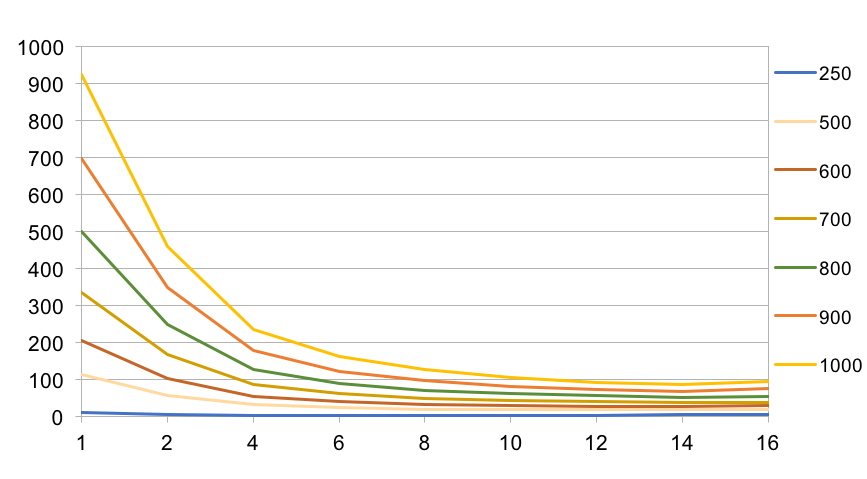
\includegraphics[width=1\linewidth, height=5cm]{V1-Timings} 
\caption{Version 1 Timings}
\label{fig:subim1}
\end{subfigure}
\begin{subfigure}{0.5\textwidth}
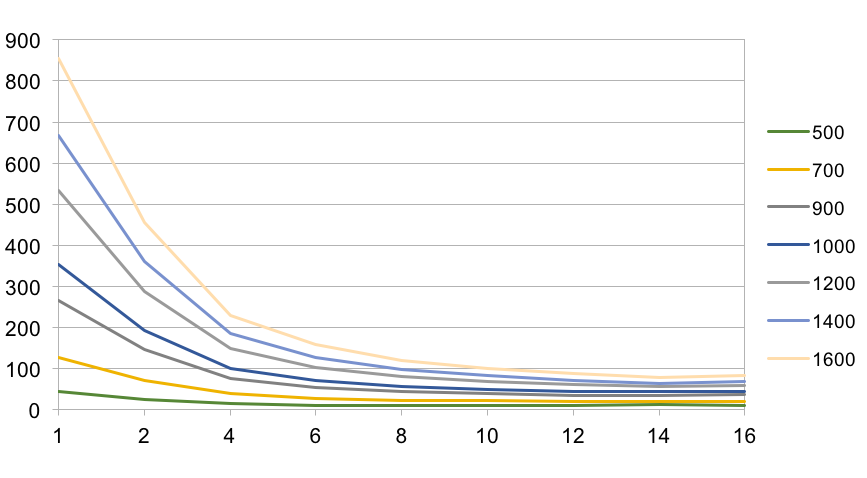
\includegraphics[width=1\linewidth, height=5cm]{V2-Timings} 
\caption{Version 2 Timings}
\label{fig:subim2}
\end{subfigure}
\caption{Version 1 and 2 Timings}
\end{figure}

\begin{figure}[h]
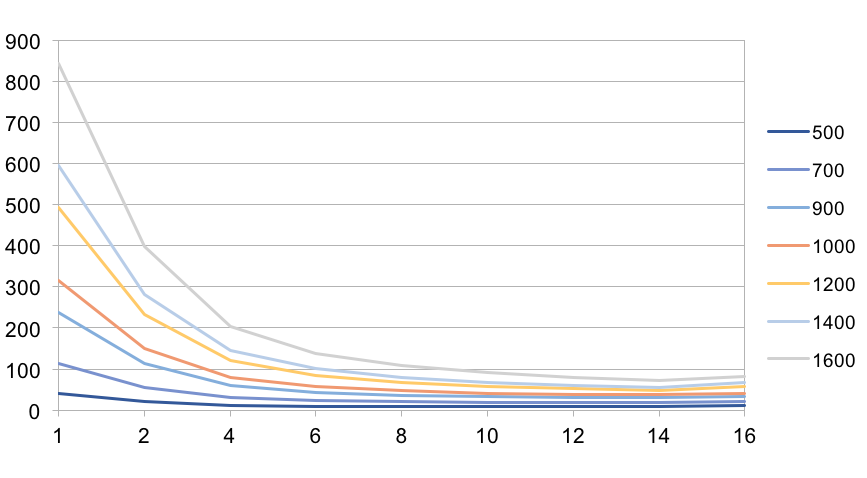
\includegraphics[width=1\textwidth]{V3-Timings}
\caption{Version 3 Timings}
\label{fig:subim3}
\end{figure}
\pagebreak
\section{Speedup}
Using the timing results that I gathered, I was able to calculate speedup for different values of p, at different problem sizes. As you can see in Figures 3.3 and 3.4, all of the parallel algorithms start off slower than than the sequentail, however by array size 250x250, all of them have speedup greater than one and so are finishing faster than their respective sequential algorithm. With some of the smaller processor counts you can see the speedup starts to level off. This is because of the Amdahl's law, which says that:
\begin{quote}
"Every program has a natural limit on the maximum speedup it can attain, regardless of the number of processors used"
\end{quote}
Unfortunately as there is a time limit for how long a program can run on balena for, we are unable to see where some of the larger threads counts speedup's level off. However as Gustafson's Law says, as the problem sizes get bigger, the sequential part effectively becomes smaller. Therefore I expect that if I was to be able to test larger problem sizes, the larger thread counts would continue to speedup.
\\\\
One oddity with my results is that for the problem sizes I was able to test, allowing the program to use 14 threads and even sometimes 12 threads, often outperforms the program that was allowed to use 16 threads. Initially I thought that I had made a mistake and was spawning one too many threads, however some simple testing by having each thread print out their thread ID, it was easy to show that this was not the case. It may be that if I was to continue to increase the problem size, 16 threads would eventually catch up and overtake them, however I was unable to test this hypotheses. 
\\\\
Finally, in a few cases the program actually gets superlinear speedup, for example for two, four and six threads of my final. This can bee seen in Figure 3.4 where the speedup lines go slightly above what you would expect their max speedup to be. There could be a few reasons for this, including that the sequential and parallel algorithms are fundamentally different, data is being more efficiently loaded into memory or there are slight variations in the time to run, that happens to cause superlinear speedup in some cases. I am pretty confident that both my sequential and parallel algorithms are so similar that this could not be the cause. While I tested the programs with cachegrind, the results did not show any noticable difference between how data was being pre-fetched for the single and parallel algorithms. However, due to how cachegrind works with multi-threaded programs, the results may not be as accurate compared to a single threaded program. Therefore I am unable to rule out how data is being pre-fetched as a reason for the slight superlinearity. On top of this, while running retests on Version 1, I noticed that even for the single threaded algorithm, there was slight differences in the time it took to run each time, which could also account for the small ammount of superlinear behaviour. Finally, as this superlinear behaviour is most prominent in my third version, there could be some intrinsic behaviour of AVX such as a warmup time that I do not know about and so have not taken into account.
\begin{figure}[h]
\begin{subfigure}{0.5\textwidth}
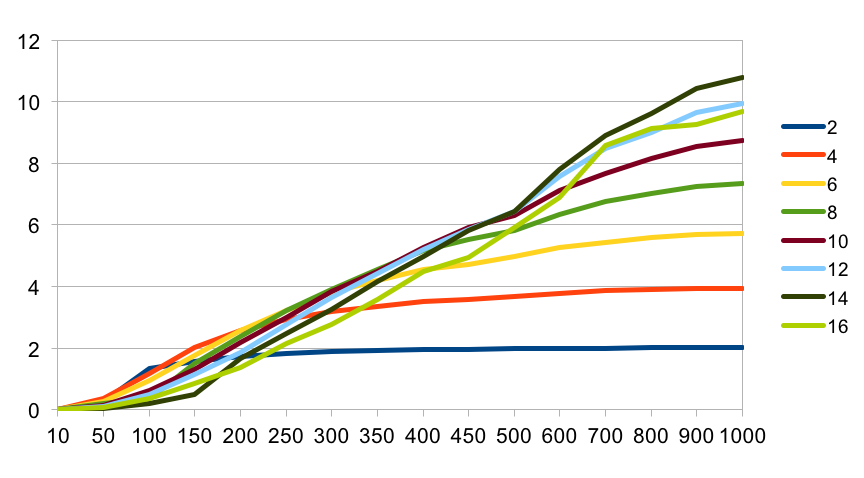
\includegraphics[width=1\linewidth, height=5cm]{V1-Speedup} 
\caption{Version 1 Timings}
\label{fig:subim4}
\end{subfigure}
\begin{subfigure}{0.5\textwidth}
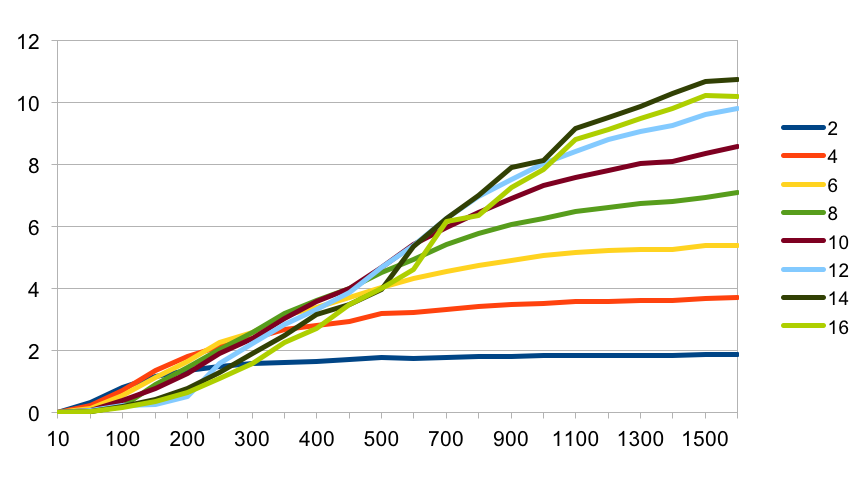
\includegraphics[width=1\linewidth, height=5cm]{V2-Speedup} 
\caption{Version 2 Timings}
\label{fig:subim5}
\end{subfigure}
\caption{Version 1 and 2 Timings}
\end{figure}
\begin{figure}[h]
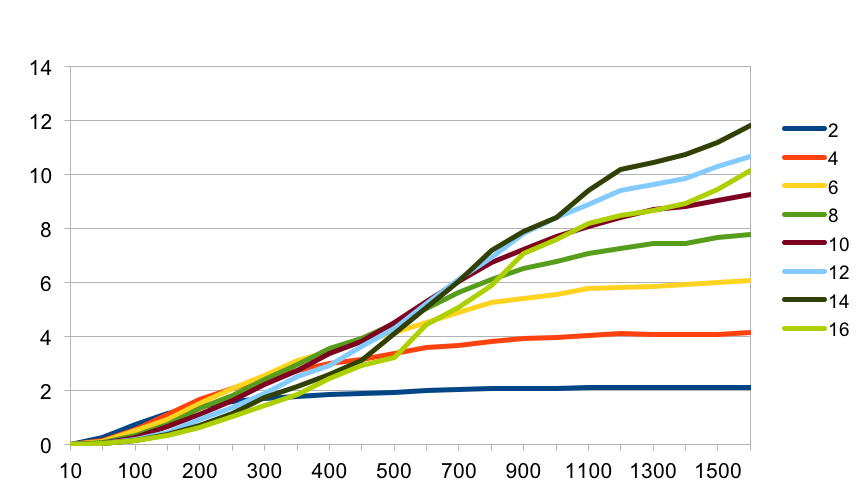
\includegraphics[width=1\textwidth]{V3-Speedup}
\caption{Version 3 Timings}
\label{fig:subim6}
\end{figure}

\section{Efficiency}
As stated earlier, efficiency is a measure of how efficiently my parallel algorithm is using the extra processors. For example, if a program has an efficiency of 0.5 for a given problem size an number of processors, then half of the time that the processors could be doing work, is lost to overheads. These graphs show that my algorithms scale pretty as efficiency increases as the problem size does. Another way thinking about this, is that with larger problem sizes, the efficiency decreases slower as the core count increases . This follows the reasoning of Gustafson's law. One thing to note, is that for some problem sizes and processor counts, V3 has lower efficiency than V1. However as V3 is so much faster than V1, I don't think this is much of an issue. Finally, these graphs more easily show the superlinear behaviour that was discussed in section 3.2, 1as efficiency can be seen going above 1.
\begin{figure}[h]
\begin{subfigure}{0.5\textwidth}
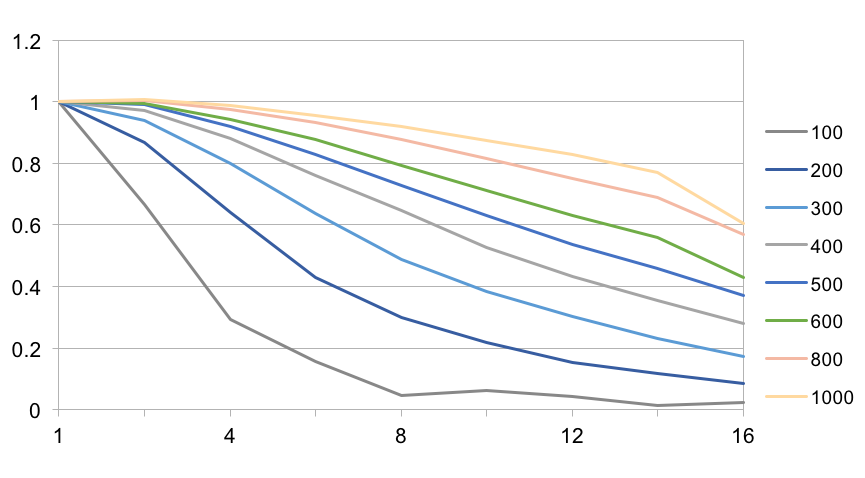
\includegraphics[width=1\linewidth, height=5cm]{V1-Efficiency} 
\caption{Version 1 Efficiency}
\label{fig:subim4}
\end{subfigure}
\begin{subfigure}{0.5\textwidth}
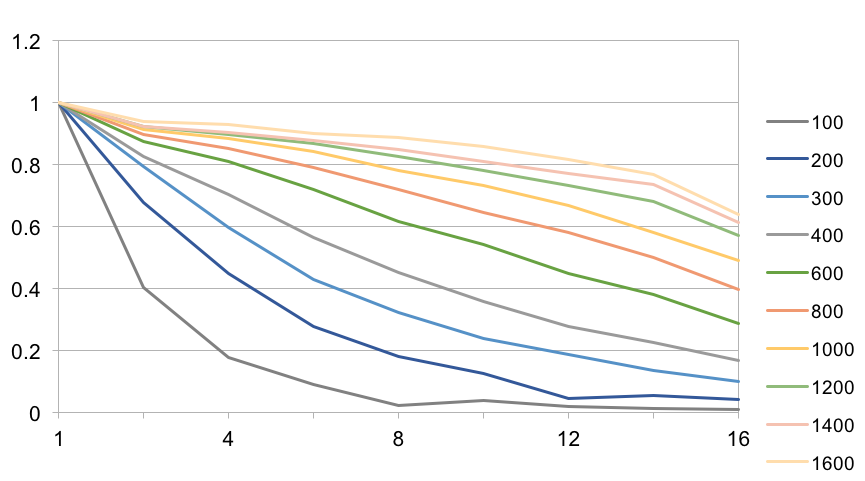
\includegraphics[width=1\linewidth, height=5cm]{V2-Efficiency} 
\caption{Version 2 Efficiency}
\label{fig:subim5}
\end{subfigure}
\caption{Version 1 and 2 Efficiency}
\end{figure}
\begin{figure}[h]
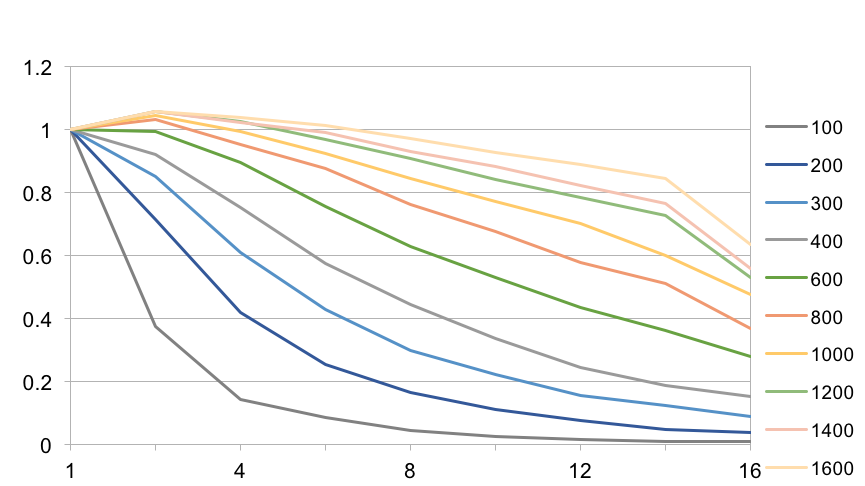
\includegraphics[width=1\textwidth]{V3-Efficiency}
\caption{Version 3 Efficiency}
\label{fig:subim6}
\end{figure}

\section{Karp-Flatt Metric}
Figures 3.7 and 3.8 show the Karp-Flatt metric of my algorithms at various array sizes. As the problem size increases, the Karp-Flatt metric decreases. This is consistent with Gustafson's law, which says that as the problem size increases, the effective sequential part of an algorithm decreases. In some of the tests, the Karp-Flatt metric is more than one as 
\begin{figure}[h]
\begin{subfigure}{0.5\textwidth}
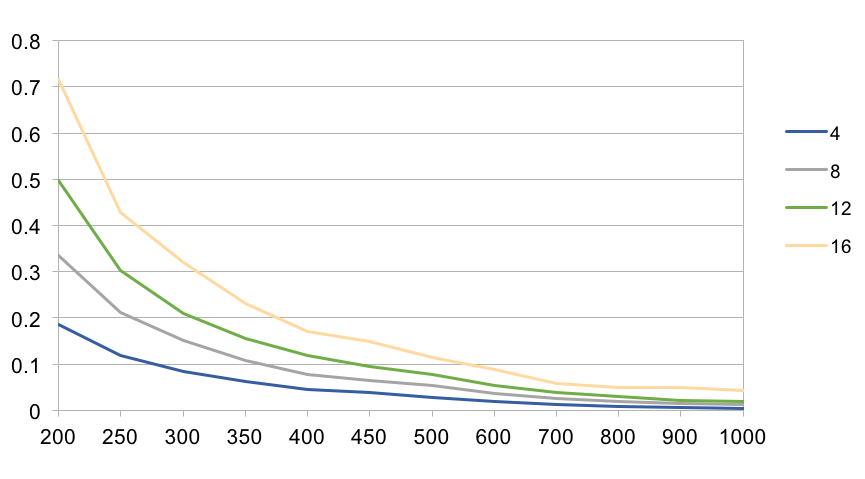
\includegraphics[width=1\linewidth, height=5cm]{V1-Karp-Flatt} 
\caption{Version 1 Karp-Flatt}
\label{fig:subim4}
\end{subfigure}
\begin{subfigure}{0.5\textwidth}
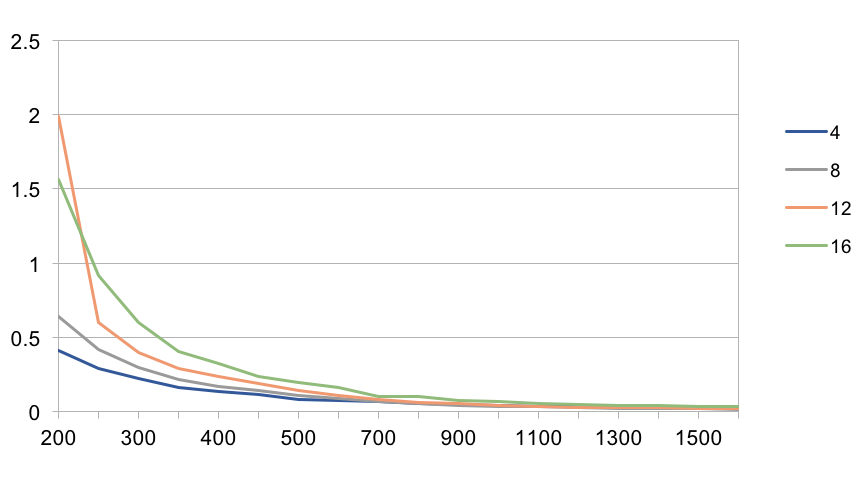
\includegraphics[width=1\linewidth, height=5cm]{V2-Karp-Flatt} 
\caption{Version 2 Karp-Flatt}
\label{fig:subim5}
\end{subfigure}
\caption{Version 1 and 2 Karp-Flatt}
\end{figure}
\begin{figure}[h]
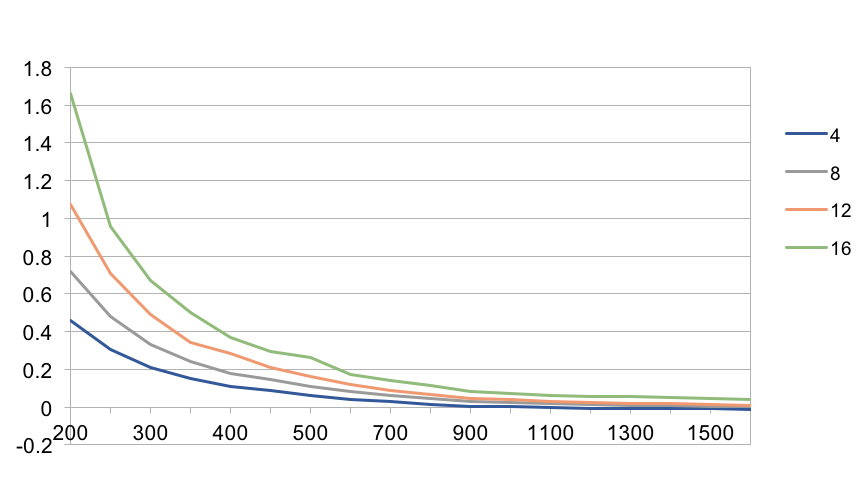
\includegraphics[width=1\textwidth]{V3-Karp-Flatt}
\caption{Version 3 Karp-Flatt}
\label{fig:subim6}
\end{figure}

\chapter{Conclusion}
My current solution scales well with core count and problem size, with the max recorded speedup being around 12. My results also show that the efficiency of my solution drops as expected, as the thread count increases. The lowest Karp-Flatt value that I messured was around 0.011. Using this value in conjunction with Amdahl's law, I can predict a max speedup of my algorithm on an array size 1600 will be around 90.
\end{document}